\documentclass[conference]{IEEEtran}
\usepackage{cite}
\usepackage{amsmath}
\usepackage{graphicx}

\title{\textbf{Peningkatan Sebuah PageRank Berbobot Untuk Menangani Persamaan Tautan Nol}}
\author{\IEEEauthorblockN{Jeremy Andika}\\
\IEEEauthorblockA{Fakultas Teknologi Informasi}\\
Institut Teknologi Batam\\
Batam, Kepulauan Riau, Indonesia\\
2022002@student.iteba.ac.id}

\begin{document}
\maketitle

% Abstract
\begin{abstract}

    Algoritma PageRank yang terkenal memanfaatkan
struktur tautan untuk menghitung peringkat kualitas halaman. Pada dasarnya ia memberikan jumlah probabilitas yang sama untuk halaman tetangga dari sebuah halaman. Sebagai ekstensi, Algoritma PageRank berbobot yang diusulkan telah memberikan perbedaan bobot untuk link keluar dari halaman. Beberapa PageRank berbobot algoritma menggunakan persamaan antar halaman sebagai bobotnya. Dalam halaman web korea, kami menemukan bahwa terkadang kebetulan memiliki nilai nol untuk persamaan antar halaman dari halaman tetangga karena karakteristik bahasa tersebut. Proposal ini mengusulkan perbaikan algoritma PageRank berbobot yang dapat menangani hal seperti antar halaman bernilai nol. Metode yang diusulkan telah diterapkan menggunakan paradigma MapReduce untuk penanganan data yang besar, dan memiliki telah dievaluasi melalui halaman web Wikipedia Korea dan dibandingkan dengan dua metode lainnya.
\end{abstract}

% Keyword
\begin{IEEEkeywords}
    PageRank; PageRank Berbobot; Persamaan; MapReduce; TFIDF
\end{IEEEkeywords}

% Introduction
\section{Pendahuluan}

Belakangan ini, ketika orang ingin mengetahui sesuatu, kebanyakan dari mereka mencoba menemukannya di Internet. Mereka akan kewalahan jika terlalu banyak halaman yang diberikan seperti halaman yang relevan dalam pencarian di web. Di pengambilan informasi \textit{(Information Retrival)}, peringkat telah menjadi salah satu masalah yang penting. Untuk memilah halaman berpengaruh dari yang dicari, berbagai peringkat algoritma telah diusulkan \cite{brin1998anatomy, xing2004weighted, qiao2010simrank, page1999pagerank, kumar2013pagerank, duhan2009page, najork2007comparing, kumar2011page, nemirovsky2008weighted, tyagi2012weighted, haveliwala2003topic}.

PageRank\cite{brin1998anatomy} merupakan salah satu algoritma peringkat terkenal yang menggunakan struktur link Web. Ini mengasumsikan bahwa seorang peselancar berjalan secara acak di atas halaman web dan mencoba untuk menentukan distribusi statis dari peselancar. Dengan penderitaan acak metafora, semakin banyak tautan yang dimiliki halaman, semakin tinggi peringkatnya. Di PageRank, yang menderita membuat jalan acak ke tetangga halaman dengan probabilitas yang sama. Kadang-kadang probabilitas yang sama ini tampaknya tidak masuk akal karena beberapa tautan terhubung ke halaman tetangga yang jauh lebih penting.

Untuk mengatasi situasi ini, algoritma PageRank berbobot \cite{xing2004weighted, qiao2010simrank,kumar2013pagerank} telah diusulkan. Mereka memperhitungkan baik distribusi jumlah in-link untuk node tetangga, jumlah kunjungan ke halaman tetangga, atau kesamaan antar halaman. Masing-masing memiliki pro dan kontra. Pembobotan berbasis kesamaan antar halaman terdengar baik untuk konten-peringkat berbasis.

Kami telah mencoba algoritma PageRank berbobot berbasis kesamaan antar halaman ke halaman Wikipedia bahasa Korea. Untuk menghitung kesamaan antar halaman, kami menggunakan model vektor \cite{}. Untuk mendapatkan representasi vektor untuk halaman, pertama-tama kami melakukan analisis morfologi untuk mengekstrak kata-kata. Berbeda dengan bahasa barat, kata benda dalam bahasa Korea menyampaikan informasi yang paling berarti. Karena karakteristik bahasa, kata benda diekstraksi untuk mengidentifikasi kata kunci. Kata kunci diidentifikasi menggunakan istilah frekuensi dan informasi frekuensi dokumen terbalik. Dengan kata kunci, representasi vektor untuk halaman diperoleh. Kemudian, kebetulan memiliki kesamaan nol ketika kesamaan antar halaman dihitung menggunakan produk dalam dari vektor tersebut. Sangat canggung untuk halaman tetangga yang tidak memiliki kesamaan. Makalah ini berkaitan dengan peningkatan PageRank berbobot berbasis kesamaan antar halaman untuk menangani kasus-kasus dengan tautan nol kesamaan.

Sisa proposal ini disusun sebagai berikut: Bagian II menyajikan PageRank dan variannya secara lebih rinci. Bagian III memperkenalkan peningkatan pada PageRank berbobot, dan Bagian IV menunjukkan beberapa hasil eksperimen untuk metode yang diusulkan. Kami menarik kenotasian di Bagian V.

% Related Works
\section{Karya yang terkait}

\subsection{Algoritma PageRank}

PageRank \cite{brin1998anatomy} adalah algoritma perbatasan yang memberi peringkat halaman dengan mengacu pada struktur tautan Web. PageRank memperlakukan halaman sebagai node dan hyperlink sebagai tepi grafik. Setiap node memiliki nilai Rank sendiri dan mendistribusikannya secara merata ke tetangganya. Distribusi berulang tanpa batas sampai semua nilai peringkat konvergen. Distribusi stasioner dari Peringkat dianggap sebagai skor Peringkat akhir halaman. Untuk mencegah peningkatan nilai Rank yang tidak terbatas, jumlah semua Rank dibatasi menjadi 1, dan juga untuk setiap nilai Rank tidak boleh lebih besar dari 1. Nilai Rank \(r_{j}\) node \(j\) dihitung sebagai berikut :
\begin{eqnarray}
    r_{j} = \sum_{i\overrightarrow{\text {out}} j}{\frac {r_{i}} {L_{out}(i)}}\\
    r_{j} = \sum r_{ i } = 1
\end{eqnarray}

Dimana \(L_{out}{(i)}\) adalah jumlah out-link dari node $i$. Setiap notasi $i$ mendistribusikan skor peringkatnya \(r_{i}\) secara merata notasi tetangganya $j$. Sebuah node $j$ mengumpulkan semua nilai Rank yang dikirim dari node tetangga dan mengambil jumlah mereka sebagai nilai Rank baru $r_{j}$. Proses distribusi rank ini dapat dinyatakan dengan matriks ketetanggaan stokastik $M$ dan vektor Rank $r$. Matriks $M$ adalah matriks yang berdekatan untuk web yang mengkodekan hubungan ketetanggaan antara halaman dan distribusi stasioner dari nilai Peringkat. Nilai Rank baru  $r^{(t+1)}$ dihitung sebagai berikut:
\begin{eqnarray}
    r^{(t+1)}=\text{M}r^{(t)}
\end{eqnarray}

di mana $t+1$ adalah langkah selanjutnya dari $t$ . Ketika semua nilai peringkat konvergen, $r^{(t+1)}$ sangat mirip dengan $r^{(t)}$. Di sini, konvergen
$r$ sesuai dengan vektor eigen dengan nilai eigen 1 untuk matriks $M$.

\subsection{Algoritma PageRank Berbobot}
Penjelajah web sebenarnya tidak melakukan asal jalan seperti di PageRank. Untuk mengakomodasi karakteristik perilaku seperti itu, pembobotan Algoritma PageRank telah diusulkan yang memungkinkan penderitaan untuk membuat transisi probabilistik yang tidak merata ke tetangga halaman \cite{xing2004weighted,qiao2010simrank,kumar2013pagerank}.

\subsubsection{PageRank berbobot berdasarkan jumlah in-link dari halaman tetangga}
Xing dan Ghorbani \cite{xing2004weighted} mengusulkan algoritma PageRank berbobot yang memberikan lebih banyak porsi Peringkat ke halaman tetangga dengan lebih banyak tautan. Hal ini memang tidak cukup mencerminkan perilaku peselancar yang sebenarnya, karena hanya informasi struktur topologi yang digunakan.

\subsubsection{PageRank Tertimbang berdasarkan Ukuran Kesamaan}
Qiaoet al. \cite{qiao2010simrank} mengusulkan varian algoritma PageRank berbobot yang disebut SimRank. Mendistribusikan ke antar-halaman yang sama, untuk menerapkan metode ini dibutuhkan infrastruktur komputasi paralel terdistribusi seperti Hadoop MapReduce.

\subsubsection{PageRank berbobot berdasarkan kunjungan tautan}
Kumaret al.\cite{kumar2013pagerank} memperkenalkan algoritma PageRank berbobot di mana node mendistribusikan lebih banyak nilai Peringkat ke tautan keluar yang lebih sering dikunjungi oleh pengguna. Algoritme ini memerlukan data klik tautan di seluruh Web. Oleh karena itu, ini sangat ideal, tetapi tidak mudah untuk menerapkannya pada skala Web.

\subsection{Algoritma Hub dan Otoritas}
Najork\cite{najork2007comparing} mengambil pendekatan yang agak berbeda dari PageRank dan mengusulkan algoritma peringkat yang disebut HITS (pencarian topik yang diinduksi hyperlink). Sementara PageRank mengasumsikan gagasan penting satu dimensi untuk halaman, HITS memandang halaman penting memiliki dua rasa kepentingan.\cite{leskovec2020mining} Oleh karena itu, algoritme menetapkan dua skor untuk setiap halaman. Halaman tertentu berharga karena memberikan informasi tentang suatu topik. Halaman-halaman ini disebut otoritas. halaman lainnya adalah 

berharga karena mereka memberi tahu Anda ke mana harus pergi untuk mencari tahu tentang topik itu. Halaman-halaman ini disebut hub. Algoritma mendefinisikan dua konsep dengan cara yang saling rekursif. Sebuah halaman dianggap sebagai hub yang baik jika terhubung ke otoritas yang baik. Sebuah halaman dianggap sebagai otoritas yang baik jika ditautkan oleh hub yang baik.\cite{leskovec2020mining}

\subsection{Komputasi Terdistribusi dan Paralel}
Pengambilan informasi dari penyimpanan data yang sangat besar, seperti Web dan penyimpanan data besar memerlukan infrastruktur komputasi yang menyimpan dan memproses data tersebut. Kami dapat menggunakan sistem superkomputer atau sistem komputasi terdistribusi dan paralel.

Hadoop\cite{dean2008mapreduce} adalah infrastruktur komputasi yang baik yang dapat dibangun dengan biaya ekonomis.
Ini adalah proyek Apache untuk platform komputasi terdistribusi yang menyediakan sistem file terdistribusi yang disebut HDFS (Hadoop Distributed File System) dan kerangka kerja komputasi paralel terdistribusi yang disebut MapReduce. Kerangka kerja MapReduce mengatur pekerjaan menjadi tugas Peta dan Mengurangi tugas. Data input dipartisi dan diproses oleh proses Map,
dan hasil pemrosesannya dibentuk menjadi pasangan nilai kunci. Hasil tugas peta diacak menjadi Kurangi tugas sesuai dengan kuncinya. Reduce proses menggabungkan nilai dengan kunci yang sama, untuk mendapatkan hasil akhir. Kerangka kerja komputasi ini memungkinkan kami untuk menangani komputasi berat seperti komputasi kesamaan halaman berpasangan.

% The Proposed Algorithm
\section{Algoritma yang Diusulkan}

PageRank berbobot berbasis kesamaan antar halaman berdasarkan kesamaan tidak dapat menangani situasi di mana kesamaan antar halaman adalah 0. Untuk mengatasi situasi ini, kami mengusulkan metode untuk menangani nol kesamaan antar halaman dan menyesuaikan bobot untuk distribusi nilai peringkat.

Kata benda-
ekstraksi kata kunci berbasis seperti di halaman Korea terkadang menemukan kata kunci umum di antara halaman yang ditautkan. Meskipun gagasan yang melekat kesamaan antar halaman untuk memperkirakan frekuensi traversal link, situasi nol-kemiripan menghambat penerapan algoritma PageRank tertimbang.

Untuk meningkatkan penerapan PageRank berbobot,
kami mengusulkan metode untuk menjamin beberapa bobot minimum dan menyesuaikan bobot. PageRank berbobot yang diusulkan bekerja sebagai berikut, yang pada dasarnya berperilaku dengan cara yang sama seperti algoritma Qiao et al.\cite{qiao2010simrank}. 

Berdasarkan ukuran kemiripan, bobot $w_{ij}$ pada simpul $i$ sampai $j$ dihitung sebagai berikut:
\begin{eqnarray}
    \text{w}_{i j}=\frac{s_{i j}}{\sum_{k \in L_{out}(i)} s_{k}}
\end{eqnarray}

di mana $s_{ij}$ adalah kesamaan antara halaman $i$ dan $j$, dan $L_{out}(i)$ menunjukkan halaman yang ditunjuk oleh halaman $i$.

Nilai peringkat $r_{j}$ halaman $j$ diperbarui, hingga peringkat semua
nilai konvergen, sebagai berikut:
\begin{eqnarray}
    r_{j}=\sum{i \in L_{i n}(j)} \beta w_{i j} r_{i}+(1-\beta) \frac{1}{N}
\end{eqnarray}

dimana $\beta$ menunjukkan tingkat teleportasi seperti di PageRank, $L_{in}(j)$ adalah halaman yang mengarah ke halaman $j$, dan $N$ adalah jumlah total halaman.

Untuk mengukur kemiripan antar halaman, kita menggunakan jarak kosinus antara vektor kata kunci yang elemennya merupakan nilai TFIDF lemma. Lemma diekstraksi dari halaman Korea menggunakan penganalisis morfologi Korea. TF (Term Frequency) adalah frekuensi lemma dalam satu halaman,
dan IDF (Inverse document frequency) adalah frekuensi halaman yang mengandung lemma.\cite{resnik1999semantic} Untuk kata kunci di halaman, TFIDF-nya dihitung sebagai berikut:
\begin{eqnarray}
    \mathrm{TFIDF}=\frac{T F}{\log \left(\frac{D F}{N}\right)}
\end{eqnarray}

Selanjutnya, kemiripan $s_{ij}$ antara halaman $i$ dan $j$ dihitung dengan jarak cosinus antara vektor kata kunci dari TFIDF vlueus:
\begin{eqnarray}
    S_{i j}=\frac{K_{i} \cdot K_{j}}{\left|K_{i}\right|\left|K_{j}\right|}
\end{eqnarray}

di mana $K_{i}$ adalah vektor kata kunci halaman $i$.

Menggunakan kesamaan dari Persamaan (7), bobot dihitung sebagai Persamaan (4). Namun, itu tidak mempertimbangkan situasi bahwa kesamaan interpage adalah nol. Oleh karena itu, kami mengusulkan sebuah algoritme, yang menanganinya dengan mengalokasikan kesamaan minimum ke tautan ke halaman dengan kesamaan nol.
\begin{eqnarray}
    \rho \frac{\min \left(s_{i j}\right)}{\sum_{L_{i n}(i)} s_{i k}}=\alpha(1-\rho) Z R
\end{eqnarray}

di mana $\rho$ adalah parameter yang disediakan pengguna untuk kesamaan nol, dan $ZR$ adalah jumlah tautan kesamaan bukan nol.

persamaan (8) dikembangkan untuk membuat bobot kemiripan yang disesuaikan dengan nol kesamaan lebih kecil dari nilai-nilai kesamaan bukan nol. $\alpha$ ditentukan menurut Persamaan. (8), di mana kesamaan minimum dikendalikan oleh $\alpha$.
Seiring dengan kesamaan baru yang disesuaikan, bobot hanya perlu dihitung ulang seperti biasa. Pada akhirnya, nilai peringkat ditentukan seperti pada algoritma PageRank berbobot dengan Persamaan (4).

\section{Percobaan}

Untuk mengevaluasi kinerjanya, kami menerapkan metode yang diusulkan untuk menentukan peringkat halaman web di Wikipedia bahasa Korea. Kami telah mengumpulkan sekitar 300.000 halaman dari Wikipedia bahasa Korea. Gambar 1 menunjukkan arsitektur sistem percobaan.

Seluruh halaman dari ko.wikipedia.org dirayapi dan disimpan ke dalam Hadoop HDFS.
Halaman-halaman diurai menggunakan penganalisis morfologi Korea untuk mengekstrak lemma. Program Hadoop MapReduce dikembangkan untuk menghitung kemunculan kata-kata di halaman. Berdasarkan data jumlah kata, TFIDFs untuk lemma setiap halaman dihitung untuk menentukan kata kunci, dan vektor kata kunci dibangun untuk setiap halaman.
Vektor kata kunci dinyatakan dengan nilai TFIDF yang dihitung. Kesamaan antara halaman tetangga dihitung menggunakan jarak cosinus. Akhirnya, nilai peringkat ditentukan oleh Persamaan (4) menggunakan bobot yang dihitung.
\begin{center}
    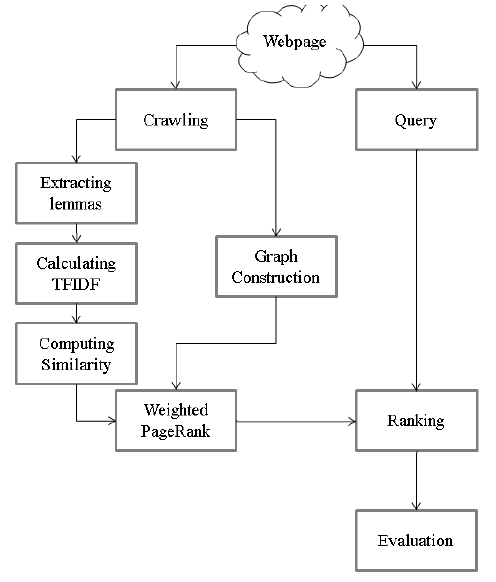
\includegraphics[scale=0.5]{chart}

Fig. 1. Arsitektur Sistem Eksperimen
\end{center}

Dalam percobaan, kami menggunakan cluster Hadoop dari 5 node untuk menangani volume data yang besar. Semua tugas dari metode yang diusulkan telah diimplementasikan dalam program MapReduce.
Kami melakukan percobaan 10 kali untuk 10 kata kunci yang dipilih secara acak dari Wikipedia dan menemukan halaman yang berisi kata kueri dan mengurutkannya menurut urutan penurunan nilai peringkatnya. Kemudian kami memilih 20 halaman teratas dan mengevaluasi relevansinya dengan 5 skala level.
Kami menghitung Normalized Discounted Cumulative Gain(NDCG)\cite{resnik1999semantic} untuk 20 halaman teratas untuk setiap kueri. NDCG adalah metrik evaluasi yang digunakan untuk mengevaluasi kinerja mesin pencari web. Ini memberikan nilai dari 0,0 hingga 1,0, dan nilai 1,0 adalah peringkat ideal entitas.
Halaman kebenaran dasar untuk kueri ditentukan dengan memilih halaman tautan keluar dari halaman kueri dalam urutan penurunan kesamaan.

Gambar 2 menunjukkan hasil eksperimen untuk PageRank asli, Qias et al.\cite{qiao2010simrank} metode dan metode yang diusulkan dalam hal NDCG.
Diamati bahwa metode yang diusulkan telah memberikan peningkatan sekitar 2 rata-rata di atas PageRank asli. Selama Qias et al.\cite{qiao2010simrank}, metode yang diusulkan meningkat pada NDCG sekitar 1,3.

Dari percobaan, kami mengamati bahwa metode yang diusulkan menghasilkan hasil yang sedikit lebih baik secara rata-rata dibandingkan dengan metode lainnya.
\begin{center}
    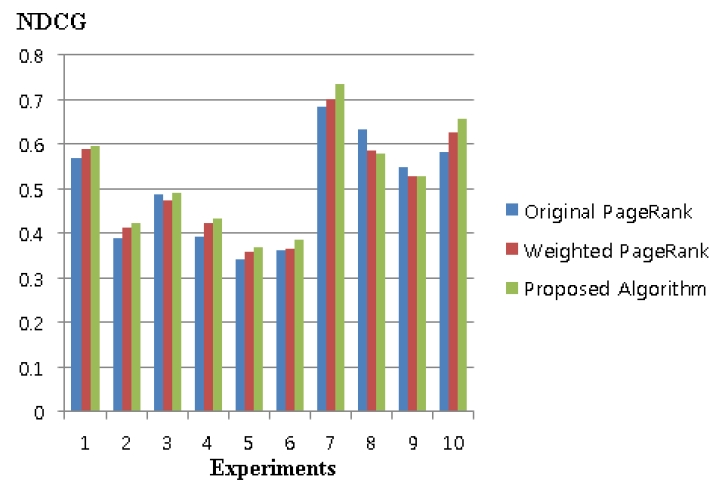
\includegraphics[scale=0.46]{graph}

Fig. 2. Perbandingan PageRank asli dan Algoritma yang diusulkan
\end{center}
% Conclusions
\section{Kesimpulan}

Dalam studi ini, kami menganalisis perilaku algoritma PageRank berbobot dan mengidentifikasi bahwa algoritma PageRank berbobot berbasis antar-kemiripan tidak dapat bekerja dengan baik dalam beberapa situasi, terutama, ketika kata kunci kata benda diekstraksi dari halaman Korea untuk perhitungan kesamaan.
Varian baru dari algoritma PageRank berbobot diusulkan untuk menangani nol kesamaan antar halaman. Untuk pemrosesan data volume besar, algoritma yang diusulkan diimplementasikan dalam program MapReduce dan kumpulan data eksperimental diproses pada cluster Hadoop dari 5 node.
Algoritma yang diusulkan telah diterapkan ke Wikipedia Korea untuk evaluasi kinerja. Dalam percobaan, kami menerapkan tiga algoritme: PageRank asli, PageRank berbobot Qias dkk.\cite{qiao2010simrank}, dan metode yang diusulkan.
Dari percobaan kami telah mengamati metode yang diusulkan mencapai beberapa perbaikan dalam hal NDCG dibandingkan metode yang dibandingkan.

\section{Pernyataan Resmi}
Penelitian ini didukung oleh MSIP (Kementerian Sains, ICT dan Perencanaan Masa Depan), Korea, di bawah program dukungan ITRC (Pusat Penelitian Teknologi Informasi) (NIPA-2013-H0301-13-4009) yang diawasi oleh NIPA (Industri TI Nasional). Agensi Promosi)

\bibliographystyle{IEEEtran}
\bibliography{references}
\end{document}